% Uncomment this to make slides with overlays:
\documentclass[slides]{beamer}

% Uncomment these (but comment the above \documentclass line) to make handouts:
%\documentclass[handout]{beamer}

% Uncomment these to have more than one slide per page
%\usepackage{pgfpages}
%\pgfpagesuselayout{2 on 1}[border shrink=5mm]
%\pgfpageslogicalpageoptions{1}{border code=\pgfusepath{stroke}}
%\pgfpageslogicalpageoptions{2}{border code=\pgfusepath{stroke}}

\usepackage[]{graphicx, color, hyperref}

\mode<presentation>
{
	%\usetheme[secheader]{Boadilla}
	%\usecolortheme[rgb={.835, .102,.169}]{structure}  
	\usetheme[width= 0cm]{Goettingen}
	%\setbeamercovered{transparent}
}
\setbeamertemplate{navigation symbols}{}
\setbeamertemplate{footline}[frame number]

\definecolor{blue2}{rgb}{0.278,0.278,0.729} 
\newcommand{\blue}[1]{\textcolor{blue2}{#1}}
\newcommand{\white}[1]{\textcolor{white}{#1}}
\newcommand{\red}[1]{\textcolor{red}{#1}}
\newcommand{\xbar}{\overline{x}}
\newcommand{\ybar}{\overline{y}}
\newcommand{\phat}{\widehat{p}}
\newcommand{\prob}{\mbox{Pr}}
\newcommand{\E}{\mathbb{E}}
\newcommand{\Var}{\mbox{Var}}
\newcommand{\cp}{\oplus}
\newcommand{\cm}{\circleddash}


\title{Lecture 18: t-distribution}
\author{Chapter 5.3}
\date{}


\begin{document}
%------------------------------------------------------------------------------
\begin{frame}
\titlepage
\end{frame}
%------------------------------------------------------------------------------








%------------------------------------------------------------------------------
\begin{frame}[fragile]
\frametitle{Goals for Today}

\begin{itemize}
\item Continue difference of means example:  Hypothesis testing
\item Paired Differences
\item What do we do when $n$ is small?  
\end{itemize}


\end{frame}
%------------------------------------------------------------------------------



%------------------------------------------------------------------------------
\begin{frame}[fragile]
\frametitle{Differences in Means:  Hypothesis Tests}
Recall the Cherry Run race data.  We test
\begin{itemize}
\item $H_0: \mu_w - \mu_m = 0$
\item $H_A: \mu_w - \mu_m \neq 0$
\end{itemize}
at the $\alpha=0.01$ significance level.

\vspace{0.5cm}

\pause We note
\begin{itemize}
\item The null states no difference in race times
\pause \item The two sided alternative is more \blue{conservative} than the one-sided alternative $\mu_w - \mu_m > 0$.
\end{itemize}
\end{frame}
%------------------------------------------------------------------------------




%-------------------------------------------------------------------------------
\begin{frame}
\frametitle{Hypothesis Testing Procedure}\label{ht}
We verified the conditions when looking at confidence intervals

\vspace{0.5cm}

\pause The \blue{test statistic} is the z-score of the point estimate $\xbar_1 - \xbar_2$ of $\mu_w - \mu_m$ under the null hypothesis:
\begin{eqnarray*}
z &=& \frac{\mbox{point estimate - null value}}{SE} = \frac{\xbar_1 - \xbar_2 - 0}{SE_{\xbar_w - \xbar_m}} = \frac{14.48}{2.77}\\
&=& 5.227
\end{eqnarray*}

\end{frame}
%-------------------------------------------------------------------------------




%pdf("./7.3 Paired Data + Diff of Two Mean/pvalue.pdf", width=8, height=6)
%x <- seq(-5.5, 5.5, by=0.01)
%plot(x, dnorm(x), xlab="z", type='l')
%abline(v=5.227, lwd=2, col="red")
%abline(v=-5.227, lwd=2, lty=2)
%legend("topleft",
%       legend=c("observed z-score", "just as extreme z-score"),
%       lty=c(1,2), lwd=c(2,2), col=c(2,1), bty="n"
%)
%dev.off()
%------------------------------------------------------------------------------
\begin{frame}[fragile]
\frametitle{Hypothesis Tests}
\begin{center}
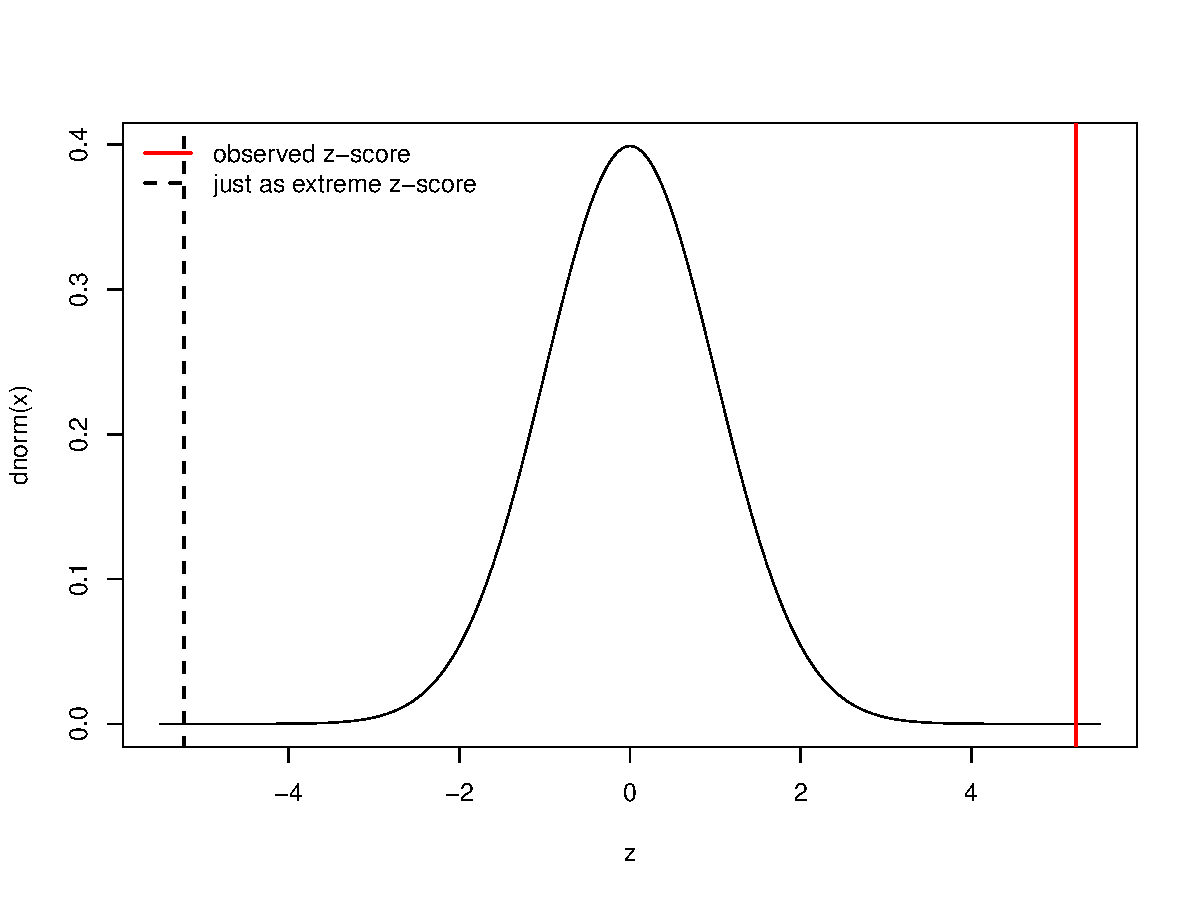
\includegraphics[width=0.7\textwidth]{pvalue.pdf}
\end{center}

\begin{enumerate}
\pause \item[4.] Compute the p-value
\begin{itemize}
\item Since the sampling distribution is normal, we use the z-table.
\item Since $H_A:  \mu_w - \mu_m \neq 0$, we have a two-sided p-value $2 \times 0 = 0$
\end{itemize}
\pause \item[5.] Since the p-value $0 < \alpha=0.01$, we reject $H_0$ and declare that men and women did not have equal mean finish times.  
\end{enumerate}





\end{frame}
%------------------------------------------------------------------------------


%------------------------------------------------------------------------------
\begin{frame}[fragile]
\frametitle{Sample Size $n$}
We need a \blue{large sample size $n$} for two reasons:

\begin{enumerate}
\item Ensure the sampling distribution of $\xbar$ is normal regardless of the true distribution by the Central Limit Theorem. 
\item ensure $s$ is a good estimate of $\sigma$, which is used in $SE = \frac{\sigma}{\sqrt{n}}$
\end{enumerate}

\pause \vspace{0.5cm}

What do we do when the sample size $n$ is small?  We're stuck, \blue{except} when 
\begin{itemize}
\item the observations are normal
\item the sample observations are independent
\end{itemize}
the sampling distribution of $\xbar$ is nearly normal \blue{regardless} of sample size $n$.


\end{frame}
%------------------------------------------------------------------------------



%------------------------------------------------------------------------------
\begin{frame}[fragile]
\frametitle{Verifying Normality}

Be cautious when verifying the normality condition for small $n$. It is important to not only examine the data but also think about where the data come from. For example, ask:
\begin{itemize}
\item Would I expect this distribution to be symmetric?
\item Am I confident that outliers are rare?
\end{itemize}

\end{frame}
%------------------------------------------------------------------------------



%-------------------------------------------------------------------------------
\begin{frame}
\frametitle{$t$ Distribution}

Let $x_1,\ldots,x_n$ be a random sample from a normal distribution.  \pause Then the standardized variable 
\[
t = \frac{\overline{x}-\mu}{SE} = \frac{\overline{x}-\mu}{\frac{s}{\sqrt n}}
\]
has probability distribution called a \blue{$t$ distribution with $n-1$ degrees of freedom ($df$)}.

\end{frame}
%-------------------------------------------------------------------------------



%%-------------------------------------------------------------------------------
%\begin{frame}
%\frametitle{$t$ Distribution}
%Extra info:  Why are they called degrees of freedom?
%
%\vspace{0.5cm}
%
%The number of degrees of freedom is the number of independent observations in a sample of data that are available to estimate a parameter of the population from which that sample is drawn. 
%
%\vspace{0.5cm}
%
%For example, if we have $n$ observations, when calculating $\xbar$ we have $n$ independent observations.  However, when calculating $s$, we use $\xbar$.  Given $\xbar$, once we've specified $n-1$ values of $x_i$, there's no more "wiggle room": everything is specified.  So $n-1$ degrees of freedom.  
%
%\end{frame}
%%-------------------------------------------------------------------------------



%-------------------------------------------------------------------------------
\begin{frame}
\frametitle{$t$ Distribution}
Properties of the $t$ distribution:

\begin{itemize}
\item a $t$-distribution has only one parameter: the \blue{degrees of freedom} $df$.
\pause \item It is bell-shaped and centered at 0, like a $z$-curve
\pause \item Any $t$ curve is more spread out than a $z$ curve.\\
i.e. it has \blue{fatter tails}
\pause \item As the $df$ goes to $\infty$, the $t$ curve approaches the $z$ curve.
\end{itemize}

\end{frame}
%-------------------------------------------------------------------------------


%-------------------------------------------------------------------------------
\begin{frame}
\frametitle{$t$ Distribution Examples}
\setkeys{Gin}{width=0.85\textwidth}
\begin{center}
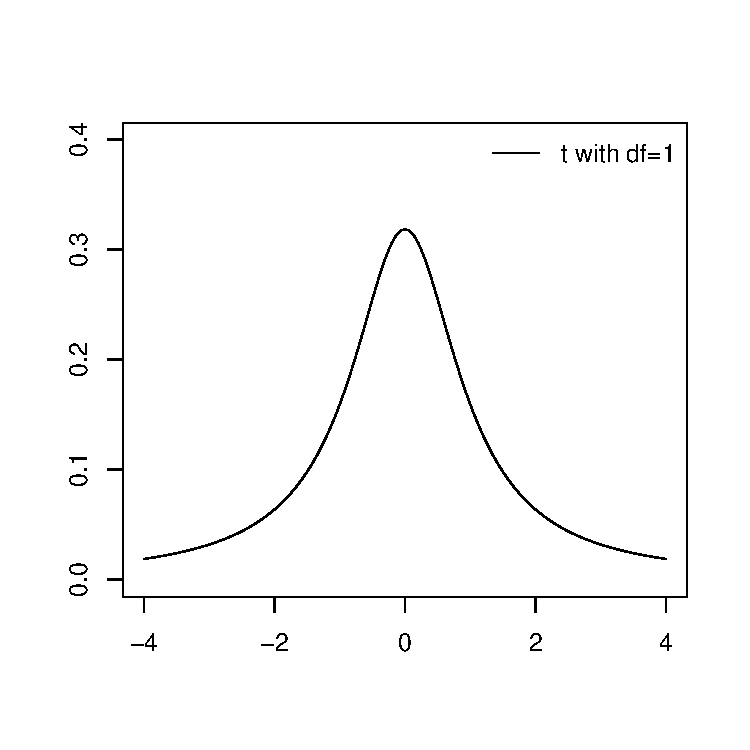
\includegraphics{lec16-001}
\end{center}
\end{frame}
%-------------------------------------------------------------------------------


%-------------------------------------------------------------------------------
\begin{frame}
\frametitle{$t$ Distribution Examples}
\setkeys{Gin}{width=0.85\textwidth}
\begin{center}
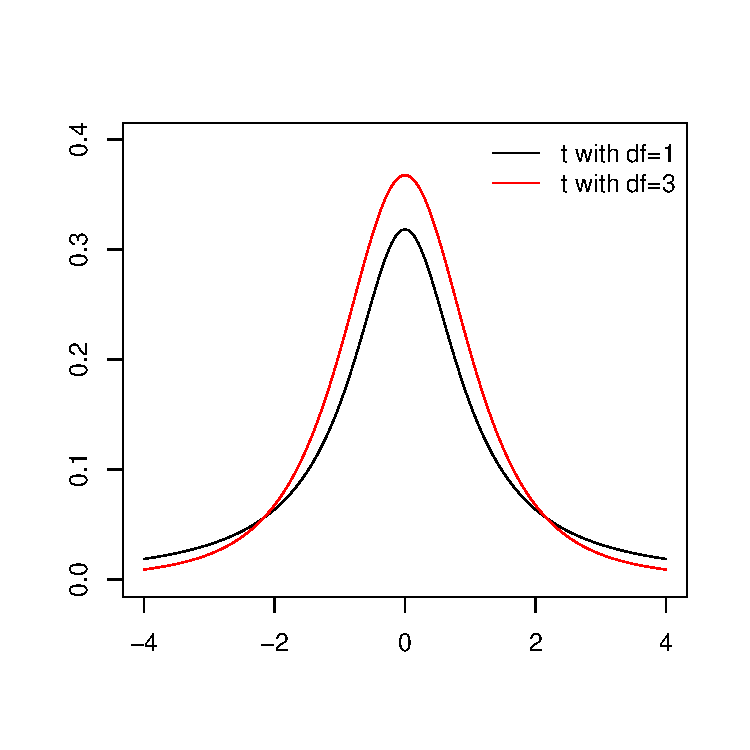
\includegraphics{lec16-002}
\end{center}
\end{frame}
%-------------------------------------------------------------------------------


%-------------------------------------------------------------------------------
\begin{frame}
\frametitle{$t$ Distribution Examples}
\setkeys{Gin}{width=0.85\textwidth}
\begin{center}
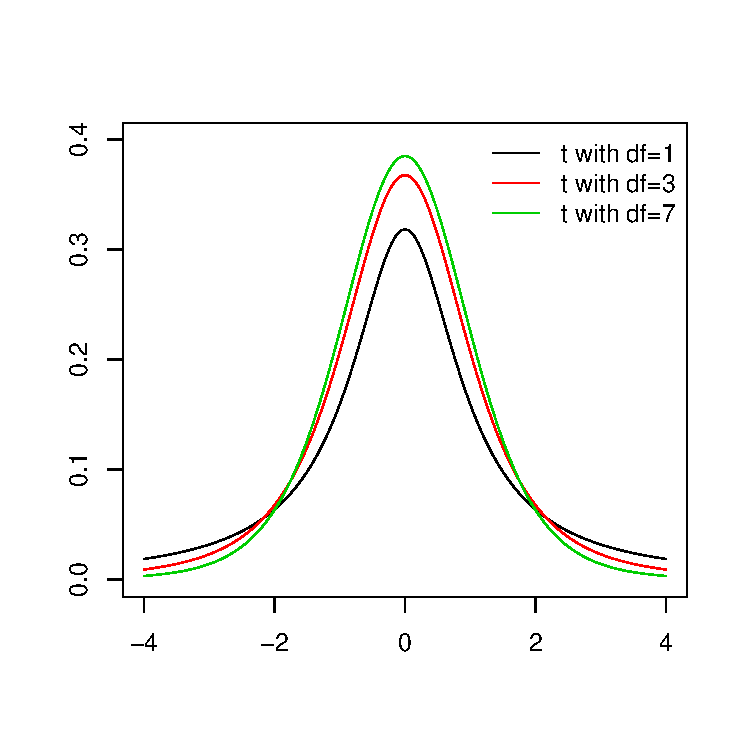
\includegraphics{lec16-003}
\end{center}
\end{frame}
%-------------------------------------------------------------------------------


%-------------------------------------------------------------------------------
\begin{frame}
\frametitle{$t$ Distribution Examples}
\setkeys{Gin}{width=0.85\textwidth}
\begin{center}
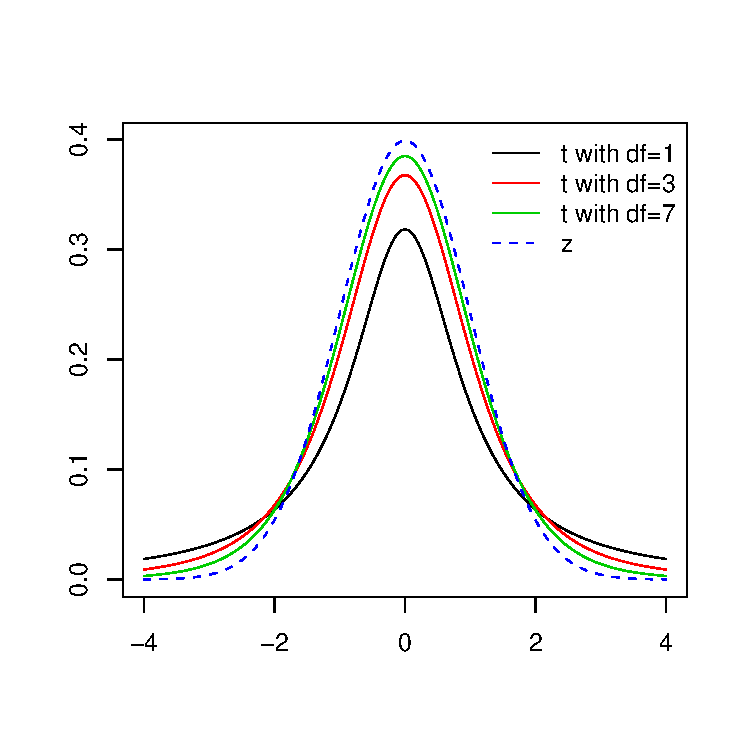
\includegraphics{lec16-004}
\end{center}
\end{frame}
%-------------------------------------------------------------------------------


%-------------------------------------------------------------------------------
\begin{frame}
\frametitle{Conditions for Using t Distribution}
We use the $t$ distribution when you have a \blue{small sample} and

\begin{itemize}
\pause \item \blue{Independence of observations}:
\begin{itemize}
\item 10\% rule on sample vs population size
\item or if we have an experiment or random process we check that each observation were independent
\end{itemize}
\pause \item \blue{Observations come from a nearly normal distribution}:  Difficult to verify with small data sets:
\begin{itemize}
\item take a look at a histogram of the data
\item consider whether any previous experiences alert us that the data may not be nearly normal
\end{itemize}
\end{itemize}  	
\end{frame}
%-------------------------------------------------------------------------------



%-------------------------------------------------------------------------------
\begin{frame}
\frametitle{$t$-Tables}
If $n=19$, we use $df=19-1=18$ and do a look up on the $t$-table on page 410:

\begin{center}
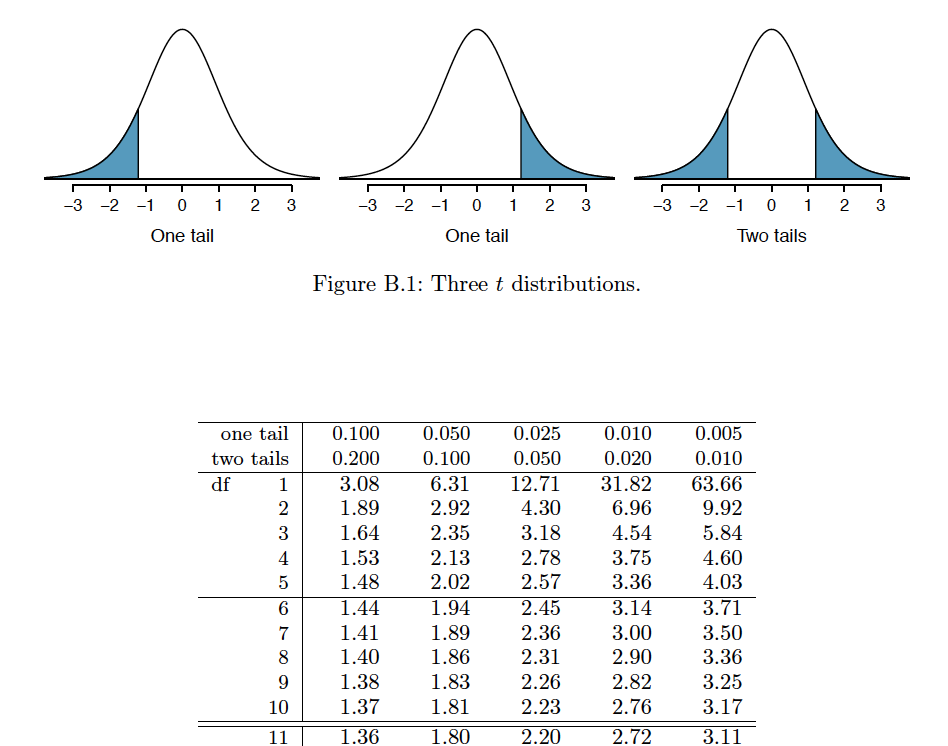
\includegraphics[width=0.75\textwidth]{t.png}
\end{center}

\end{frame}
%-------------------------------------------------------------------------------



%-------------------------------------------------------------------------------
\begin{frame}
\frametitle{Confidence Intervals}


Confidence intervals:  Use $t^*_{df}$ instead of $z^*$
\[
\left[\xbar - t_{df}^* SE, \mbox{  }\xbar + t_{df}^* SE\right] = 
\left[
\overline{x} - t_{df}^* \times\frac{s}{\sqrt n}, \mbox{  }
\overline{x} + t_{df}^* \times\frac{s}{\sqrt n}
\right]
\]


So for example, to get a 95\% C.I. based on $n=18 \Rightarrow df=17$, $t_{17}^*=2.11$.


\end{frame}
%-------------------------------------------------------------------------------




%-------------------------------------------------------------------------------
\begin{frame}
\frametitle{$t$-Test}
The $t$-test is the same as the previous test, where instead of finding the $z$-score of $\xbar$, we find the \blue{$t$-statistic/score}.

\vspace{0.5cm}

\pause Example 5.19 on page 252:  NYC is known as the city that never sleeps.  A random sample of 25 New Yorkers were asked how much sleep they get per night. Does the data below provide strong evidence that New Yorkers sleep less than 8 hours a night on average?  Set $\alpha=0.05$

\vspace{0.5cm}
\begin{center}
\begin{tabular}{c|c|c|c|c}
$n$ & $\xbar$ & $s$ & min & max\\
\hline
25 & 7.73 & 0.77 & 6.17 & 9.78\\
\end{tabular}
\end{center}

\end{frame}
%-------------------------------------------------------------------------------











%-------------------------------------------------------------------------------
\begin{frame}
\frametitle{$t$-Test}
2. Conditions:
\begin{itemize}
\item \blue{Independence}: 25 is obviously less than 10\% of the study population of NYC
\item What about normality?  Not an exact science.  The halfway point of the min and max is 7.975, which is fairly close to $\xbar=7.73$.  So symmetric enough. 
\end{itemize}

\vspace{0.25cm}

\pause 3. The test statistic is the $t$-statistic:
\[
t = \frac{\overline{x}-\mbox{null value}}{SE} = \frac{\overline{x}-\mbox{null value}}{\frac{s}{\sqrt n}} = \frac{7.73 - 8}{\frac{0.77}{\sqrt{25}}} = -1.75
\]
Since $n=25$, $df=25-1=24$.
\end{frame}
%-------------------------------------------------------------------------------



%-------------------------------------------------------------------------------
\begin{frame}
\frametitle{$t$-Test}

4. $p$-Value. We use the $t$ distribution i.e. the $t$-table on page 410:
\begin{center}
\begin{tabular}{c|ccccc}
\hline
one-tail & 0.100 & 0.050 & 0.025 & 0.010 & 0.005\\
two-tail & 0.200 & 0.100 & 0.050 & 0.020 & 0.010\\
\hline
df = 24 & 1.32 & 1.71 & 2.06 & 2.49 & 2.80\\
\hline
\end{tabular}
\end{center}

Since 1.75 is in between one-tail values of 1.71 and 2.06 and by symmetry, the p-value is somewhere between 0.05 and 0.025. 

\vspace{0.5cm}

\pause 5.  Decision: Since the p-value $< \alpha=0.05$, we reject the null hypothesis that NY'ers sleep 8 hours a night at the $\alpha=0.05$ significance level.  
\end{frame}
%-------------------------------------------------------------------------------



%-------------------------------------------------------------------------------
\begin{frame}
\frametitle{History of $t$ Distribution}
The $t$ distribution was derived by William Sealy Gosset in 1908, a chemist/statistician at the Guinness Brewery in Dublin, Ireland.
\begin{center}
\includegraphics[width=2in]{gosset.pdf}
\end{center}
\end{frame}
%-------------------------------------------------------------------------------


%-------------------------------------------------------------------------------
\begin{frame}
\frametitle{History of $t$ Distribution}
Gosset was concerned with \blue{small-sample statistics} about barley given that brewers are limited in the number of batches of beer they can brew.
\pause \vskip 0.5cm
Guinness prohibited its employees from publishing.  So Gosset had to use the pseudonym ``Student'' to conceal his identity.
\pause \vskip 0.5cm
In particular, the \blue{(Student's) t-test} is one of the most widely used statistical tests in the world.  
\end{frame}
%-------------------------------------------------------------------------------


%-------------------------------------------------------------------------------
\begin{frame}
\frametitle{History of $t$ Distribution}
In fact if you go to the Guinness Brewery at St James's Gate in Dublin, Ireland...
\begin{center}
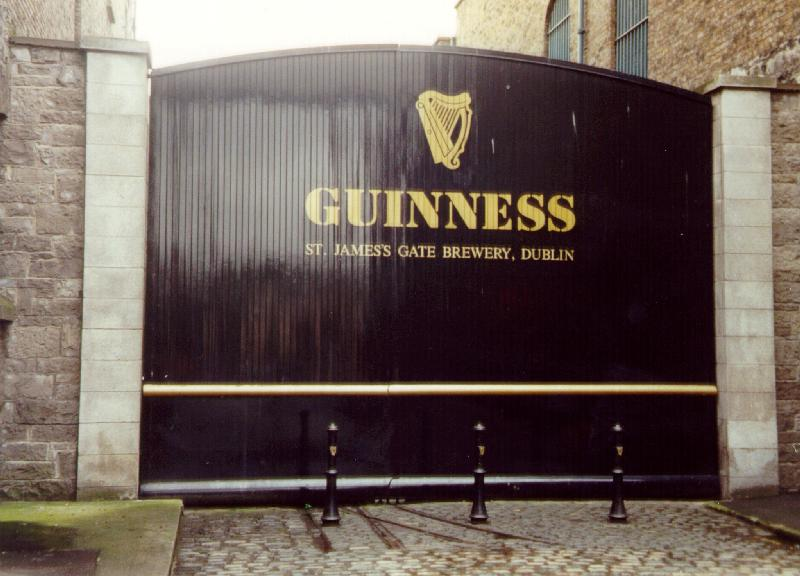
\includegraphics[width=3in]{brewery.jpg}
\end{center}
\
\end{frame}
%-------------------------------------------------------------------------------


%-------------------------------------------------------------------------------
\begin{frame}
\frametitle{History of $t$ Distribution}
\begin{center}
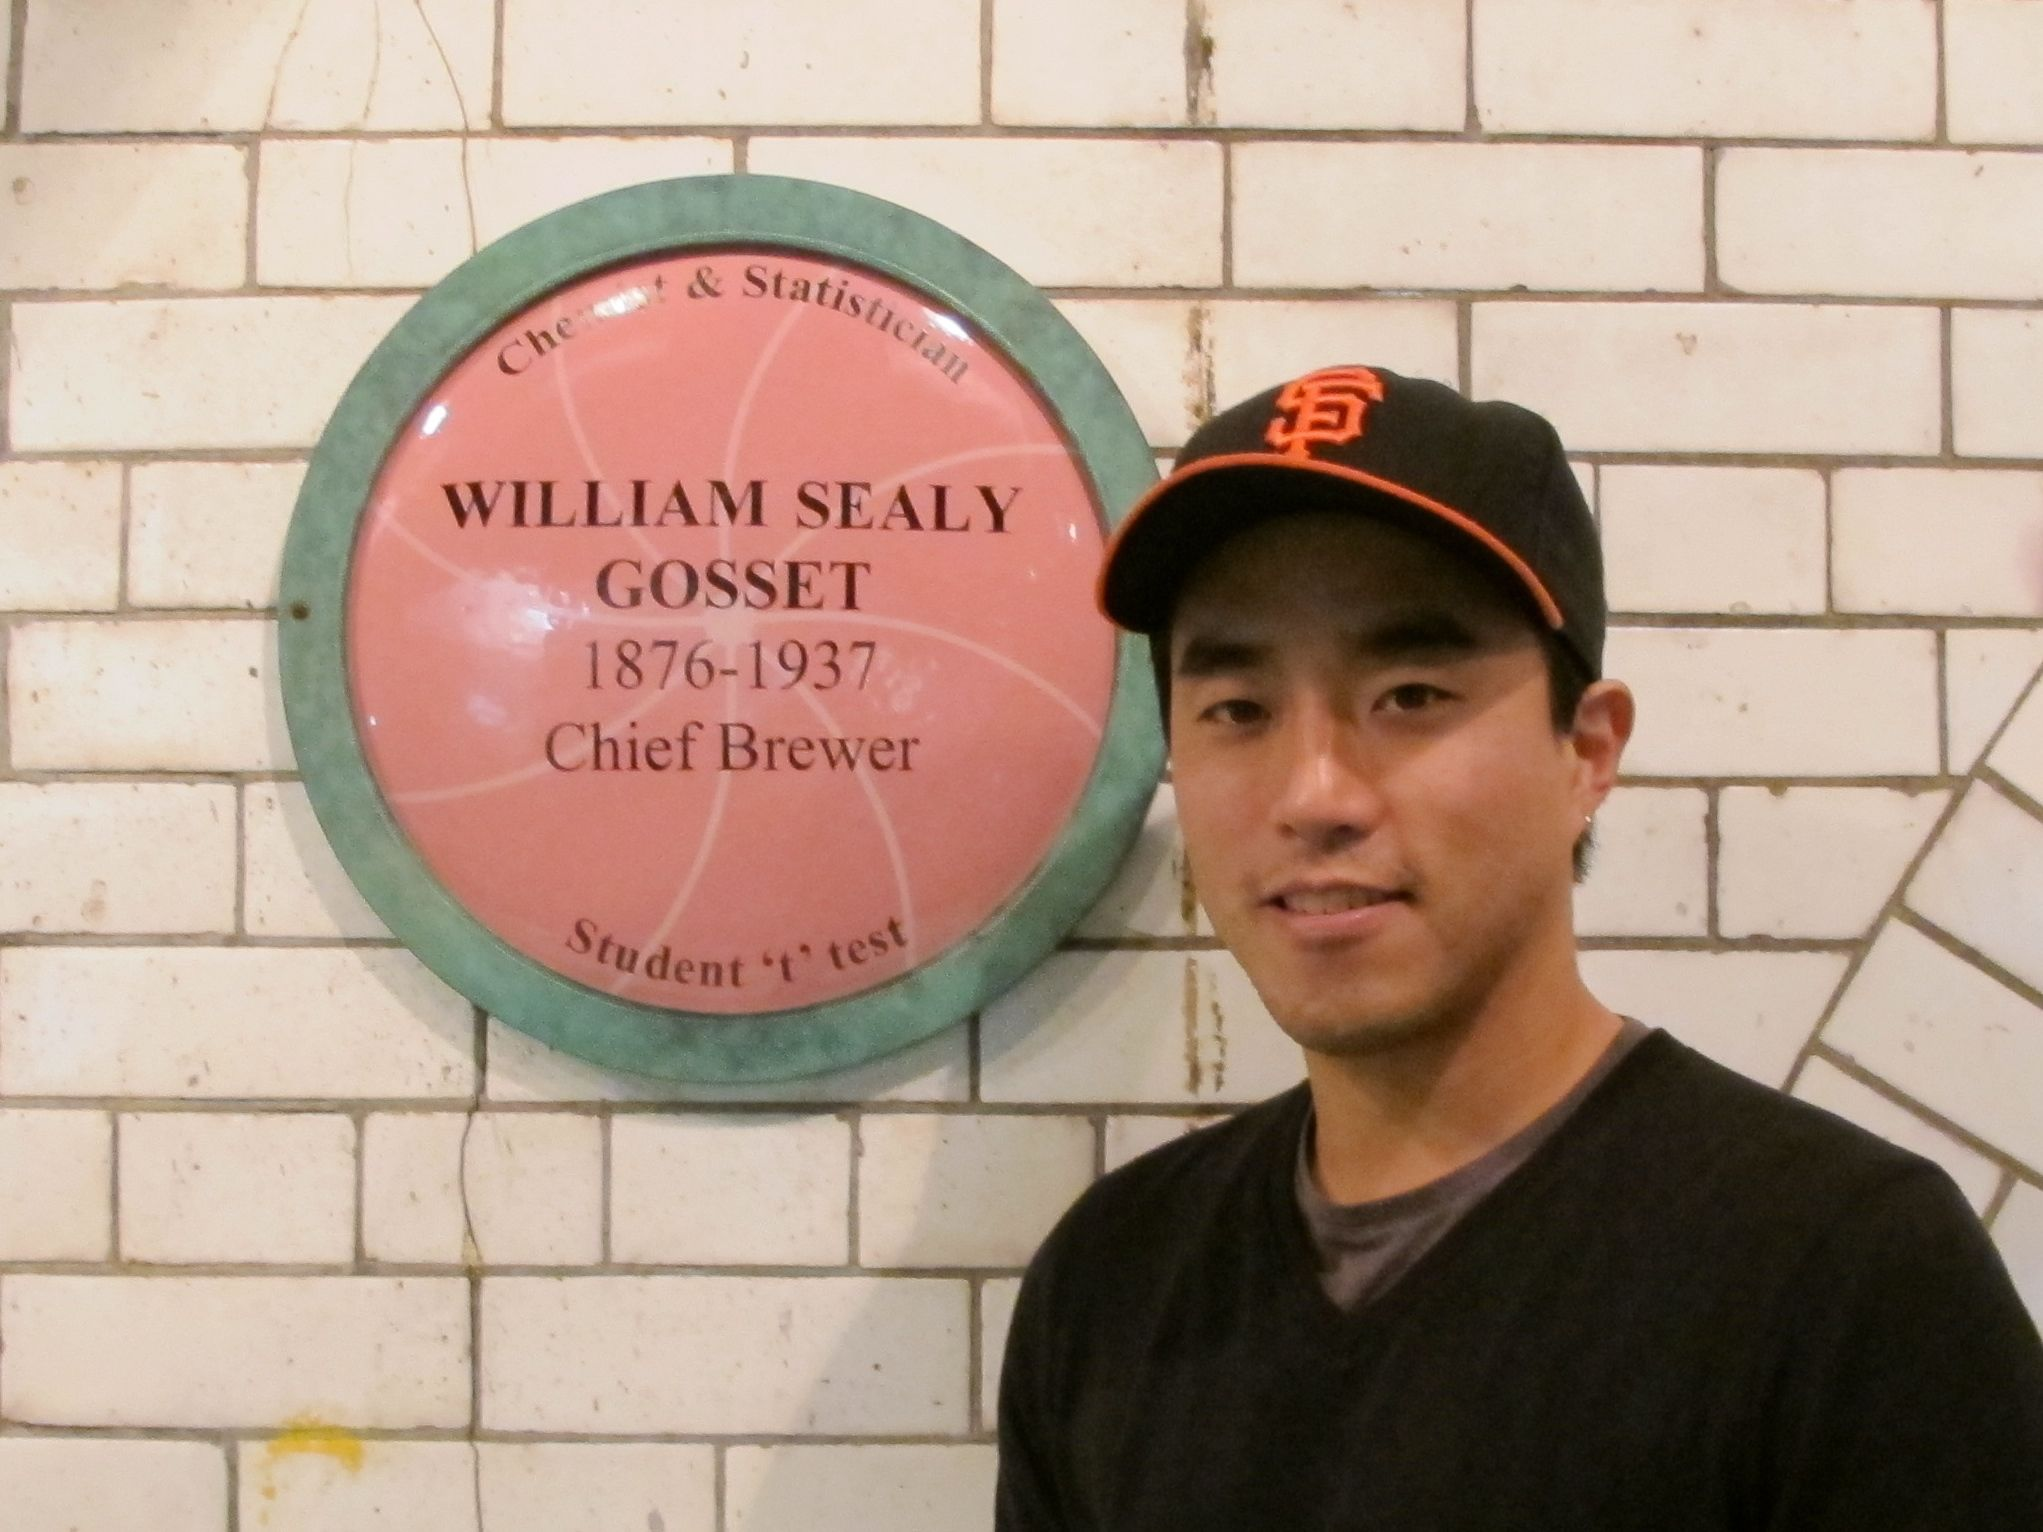
\includegraphics[width=0.9\textwidth]{guinness.jpg}
\end{center}
\end{frame}
%-------------------------------------------------------------------------------

%
%
%%------------------------------------------------------------------------------
%\begin{frame}[fragile]
%\frametitle{Next Time}
%
%Same $t$-test scenario:  small sample size with normal data, but now, differences in means $\mu_1-\mu_2$
%
%\end{frame}
%%------------------------------------------------------------------------------







\end{document}










